\documentclass[journal]{vgtc}                % final (journal style)
%\let\ifpdf\relax
%\documentclass[review,journal]{vgtc}         % review (journal style)
%\documentclass[widereview]{vgtc}             % wide-spaced review
%\documentclass[preprint,journal]{vgtc}       % preprint (journal style)

%% Uncomment one of the lines above depending on where your paper is
%% in the conference process. ``review'' and ``widereview'' are for review
%% submission, ``preprint'' is for pre-publication, and the final version
%% doesn't use a specific qualifier.

%% Please use one of the ``review'' options in combination with the
%% assigned online id (see below) ONLY if your paper uses a double blind
%% review process. Some conferences, like IEEE Vis and InfoVis, have NOT
%% in the past.

%% Please use the ``preprint''  option when producing a preprint version
%% for sharing your article on an open access repository

%% Please note that the use of figures other than the optional teaser is not permitted on the first page
%% of the journal version.  Figures should begin on the second page and be
%% in CMYK or Grey scale format, otherwise, colour shifting may occur
%% during the printing process.  Papers submitted with figures other than the optional teaser on the
%% first page will be refused. Also, the teaser figure should only have the
%% width of the abstract as the template enforces it.

%% These few lines make a distinction between latex and pdflatex calls and they
%% bring in essential packages for graphics and font handling.
%% Note that due to the \DeclareGraphicsExtensions{} call it is no longer necessary
%% to provide the the path and extension of a graphics file:
%% 
\includegraphics{diamondrule} is completely sufficient.
%%
\ifpdf%                                % if we use pdflatex
  \pdfoutput=1\relax                   % create PDFs from pdfLaTeX
  \pdfcompresslevel=9                  % PDF Compression
  \pdfoptionpdfminorversion=7          % create PDF 1.7
  \ExecuteOptions{pdftex}
  \usepackage{graphicx}                % allow us to embed graphics files
  \DeclareGraphicsExtensions{.pdf,.png,.jpg,.jpeg} % for pdflatex we expect .pdf, .png, or .jpg files
\else%                                 % else we use pure latex
  \ExecuteOptions{dvips}
  \usepackage{graphicx}                % allow us to embed graphics files
  \DeclareGraphicsExtensions{.eps}     % for pure latex we expect eps files
\fi%

%% it is recomended to use ``\autoref{sec:bla}'' instead of ``Fig.~\ref{sec:bla}''
\graphicspath{{figures/}{pictures/}{images/}{./}} % where to search for the images

\usepackage{microtype}                 % use micro-typography (slightly more compact, better to read)
\PassOptionsToPackage{warn}{textcomp}  % to address font issues with \textrightarrow
\usepackage{textcomp}                  % use better special symbols
\usepackage{mathptmx}                  % use matching math font
\usepackage{times}                     % we use Times as the main font
\renewcommand*\ttdefault{txtt}         % a nicer typewriter font
%\usepackage{cite}                      % needed to automatically sort the references
\usepackage{tabu}                      % only used for the table example
\usepackage{booktabs}                  % only used for the table example
\usepackage[numbers]{natbib}                    % for citations
\usepackage{anyfontsize}              % 
%% We encourage the use of mathptmx for consistent usage of times font
%% throughout the proceedings. However, if you encounter conflicts
%% with other math-related packages, you may want to disable it.

%% In preprint mode you may define your own headline. If not, the default IEEE copyright message will appear in preprint mode.
%\preprinttext{To appear in IEEE Transactions on Visualization and Computer Graphics.}

%% In preprint mode, this adds a link to the version of the paper on IEEEXplore
%% Uncomment this line when you produce a preprint version of the article
%% after the article receives a DOI for the paper from IEEE
%\ieeedoi{xx.xxxx/TVCG.201x.xxxxxxx}

%% If you are submitting a paper to a conference for review with a double
%% blind reviewing process, please replace the value ``0'' below with your
%% OnlineID. Otherwise, you may safely leave it at ``0''.
\onlineid{0}

%% declare the category of your paper, only shown in review mode
\vgtccategory{Research}
%% please declare the paper type of your paper to help reviewers, only shown in review mode
%% choices:
%% * algorithm/technique
%% * application/design study
%% * evaluation
%% * system
%% * theory/model
\vgtcpapertype{vgtcpapertype here}

%% Paper title.
\title{Absence Makes The Chart Grow Stronger: Blank Space and Axis Range Influence Interpretations of Magnitude in Risk Communication}

%% This is how authors are specified in the journal style

%% indicate IEEE Member or Student Member in form indicated below
\author{Duncan Bradley, Gabriel Strain, Caroline Jay, Andrew J. Stewart}
\authorfooter{
%% insert punctuation at end of each item
\item{Duncan Bradley is with the Division of Neuroscience and Experiment Psychology, The University of Manchester, UK. Email: duncan.bradley@manchester.ac.uk.}
\item{Gabriel Strain and Caroline Jay are with the Department of Computer Science, The University of Manchester, UK. Email: \{gabriel.strain \textbar{} caroline.jay\}@manchester.ac.uk.}
\item{Andrew J. Stewart is with the Division of Neuroscience and Experiment Psychology and the Department of Computer Science, The University of Manchester, UK. Email: andrew.stewart@manchester.ac.uk.}
}

%other entries to be set up for journal
\shortauthortitle{Duncan Bradley \MakeLowercase{\textit{et al.}}: Absence Makes The Chart Grow Stronger}
%\shortauthortitle{Firstauthor \MakeLowercase{\textit{et al.}}: Paper Title}

%% Abstract section.
\abstract{When visualizing data, chart designers have the freedom to choose the upper and lower limits of their numerical axes. Axis limits determine the physical positions of plotted values, and can introduce substantial blank space. For charts presenting data on the chance of negative events occuring, manipulating axis limits affects viewers' interpretations of plotted values' magnitudes, influencing understanding of the risk information being communicated. Across three experiments (total N=420), we demonstrate that, surprisingly, participants did not simply equate values presented at higher vertical positions with greater magnitudes. Instead, they used the numerical context supplied by axis limits to assess the magnitude of data points by contrasting these values against accompanying blank space. Data points were considered larger when they were numerically greater than the plausible values implied by blank space, \emph{even} when they were presented at the \emph{bottom} of a chart. Chart designers must consider the role of their axis range in viewers' interpretations of the magnitudes of plotted data points. We recommend displaying the range of relevant values in order to communicate the specific context for each dataset.} 

%% Keywords that describe your work. Will show as 'Index Terms' in journal
%% please capitalize first letter and insert punctuation after last keyword
\keywords{Cognition, framing effects, chart design, axis range, magnitude judgements.}

%% ACM Computing Classification System (CCS).
%% See <http://www.acm.org/class/1998/> for details.
%% The ``\CCScat'' command takes four arguments.

\CCScatlist{ % not used in journal version
 \CCScat{code here}{title here}%
}

%% A teaser figure can be included as follows
%\teaser{
%  \centering
%  \includegraphics[width=\linewidth]{CypressView}
%  \caption{caption here}
%  \label{fig:teaser}
%}

%% Uncomment below to disable the manuscript note
%\renewcommand{\manuscriptnotetxt}{}

%% Copyright space is enabled by default as required by guidelines.
%% It is disabled by the 'review' option or via the following command:
% \nocopyrightspace


\vgtcinsertpkg

%%%%%%%%%%%%%%%%%%%%%%%%%%%%%%%%%%%%%%%%%%%%%%%%%%%%%%%%%%%%%%%%
%%%%%%%%%%%%%%%%%%%%%% START OF THE PAPER %%%%%%%%%%%%%%%%%%%%%%
%%%%%%%%%%%%%%%%%%%%%%%%%%%%%%%%%%%%%%%%%%%%%%%%%%%%%%%%%%%%%%%%%

\begin{document}

%% The ``\maketitle'' command must be the first command after the
%% ``\begin{document}'' command. It prepares and prints the title block.

%% the only exception to this rule is the \firstsection command
\firstsection{Introduction}

\maketitle

%% \section{Introduction} %for journal use above \firstsection{..} instead

{Context is crucial for effectively judging the magnitude of numbers. A 40\% probability is twice as great as a 20\% probability, but in the absence of context, it is unclear whether this value should be considered large or small. For the chance of experiencing post-surgery complications, 40\% may be considered large, but may be considered small for the chance that a laboratory test can detect a disease.

In charts, numerical axes often provide contextual cues for judging the magnitude of plotted values. The range of values on an axis provides a frame of reference for assessing whether a data point is numerically large or small. Figure \ref{fig:senators-chart} (a reproduction of a bar chart from the New York Times), which plots over time the number of Black members of the U.S. senate \citep{history_art__archives_us_house_of_representatives_office_of_the_historian_black-american_nodate}, provides a striking illustration. Unusually, the continuous y-axis does not terminate just above the highest plotted value. Instead, it extends all the way to the maximum possible number of senators: 100. As a result, bars representing Black senators are confined to the very bottom, visible just above the x-axis, and a significant expanse of blank space looms above them. This highlights the absent data points: the vast majority of senators who are not Black. The visual arrangement communicates the magnitude of the plotted values in context.

It is unclear exactly how an axis range influences a viewer's inferences about magnitude. One possible explanation is that the unfilled area indicates the range of plausible values. That is, plotted values may be judged as small in magnitude because the potential for substantially larger values is clearly displayed. Alternatively, viewers' assessments may be influenced by the appearance of plotted values only, and not by contrast with blank space. Viewers may simply interpret the magnitude of data points at higher positions as `high' and those at lower position as `low', ignoring the plausible alternative values implied by blank space. The present set of experiments explores which of these two accounts explains how axis ranges contribute to the communication of magnitude.}

\hypertarget{effects-of-context-on-magnitude-judgments}{%
\subsection{Effects of Context on Magnitude Judgments}\label{effects-of-context-on-magnitude-judgments}}

Empirical evidence demonstrates that judgment of a value's magnitude can
depend on its relationship to a grand total or to surrounding values.
This can influence interpretation of verbal approximations, and also
absolute values. For example, participants instructed to take `a few'
marbles picked up more when the total number available was larger
(\citep{borges_common_1974}) and rated satisfaction with the same salary as
higher when it appeared in the upper end of a range, compared to the
lower end \citep{brown_does_2008}.~

\hypertarget{effects-of-axis-limits-on-comparison-of-values}{%
\subsection{Effects of Axis Limits on Comparison of Values}\label{effects-of-axis-limits-on-comparison-of-values}}

Several studies have explored how axis limits can alter impressions of
the \emph{relationships between} presented values, rather than the magnitudes
of values themselves. When axis ranges are expanded to create blank
space around a cluster of data points, correlation between those points
is judged as stronger \citep{cleveland_variables_1982}. In bar charts,
participants rate the differences between values as greater when the
vertical gap between bars is larger, due to a truncated y-axis
\citep{pandey_how_2015}. Correll et al.'s \citep{correll_truncating_2020}
experiments found that greater truncation resulted in higher effect-size
judgments in both line charts and bar charts. Truncation effects
persisted even when participants estimated the values of specific data
points, suggesting this bias is driven by initial impressions, rather
than a misinterpretation of the values portrayed by graphical markings.
\citet{correll_truncating_2020} found no reduction in effect size judgments
when truncation was communicated using graphical techniques (e.g., axis
breaks and gradients). The unavoidable consequence, they suggest, is
that designers' choices will influence viewers' interpretations whether
axes are truncated or not.

Choosing an appropriate axis range involves a trade-off between
participants' bias (over-reliance on the visual appearance of
differences) and their sensitivity (capacity to visually recognize
actual differences). Just as a highly truncated y-axis can exaggerate
trivial differences between values, an axis spanning the entire range of
possible values can conceal important differences \citep{witt_graph_2019}.
Based on participants' judgments of effect size, \citet{witt_graph_2019} found
that bias was reduced and sensitivity increased when using an axis range
of approximately 1.5 standard deviations of the plotted data, compared
to axes which spanned only the range of the data, or the full range of
possible values. This provides further evidence of a powerful
association between the appearance of data, when plotted, and subjective
interpretations of differences between data points.

Further evidence of truncation effects, provided by
\citet{yang_truncating_2021} improves on the design of previous studies which
employed only a few observations per condition \citep{pandey_how_2015} or
very small sample sizes \citep{witt_graph_2019}. Participants' ratings of
the difference between two bars consistently provided evidence of the
exaggerating effects of y-axis truncation. \citet{yang_truncating_2021} noted
that increasing awareness does not eliminate the effect, which may
function like an anchoring bias, where numerical judgments are
influenced by reference points \citep{tversky_judgment_1974}. Another
potential explanation discussed draws upon Grice's cooperative principle
\citep{grice_logic_1975}. According to this account of effective
communication, speakers are assumed to be in cooperation, and so will
communicate in a manner that is informative, truthful, relevant, and
straightforward. Analogously, a viewer will assume that a numerical
difference in a chart must be genuinely large if it appears large, else
it would not be presented that way. Effective visualizations should be
designed so a viewer's instinctive characterization of the data
corresponds closely to their interpretation following a more detailed
inspection \citep{yang_truncating_2021}.

\begin{figure}
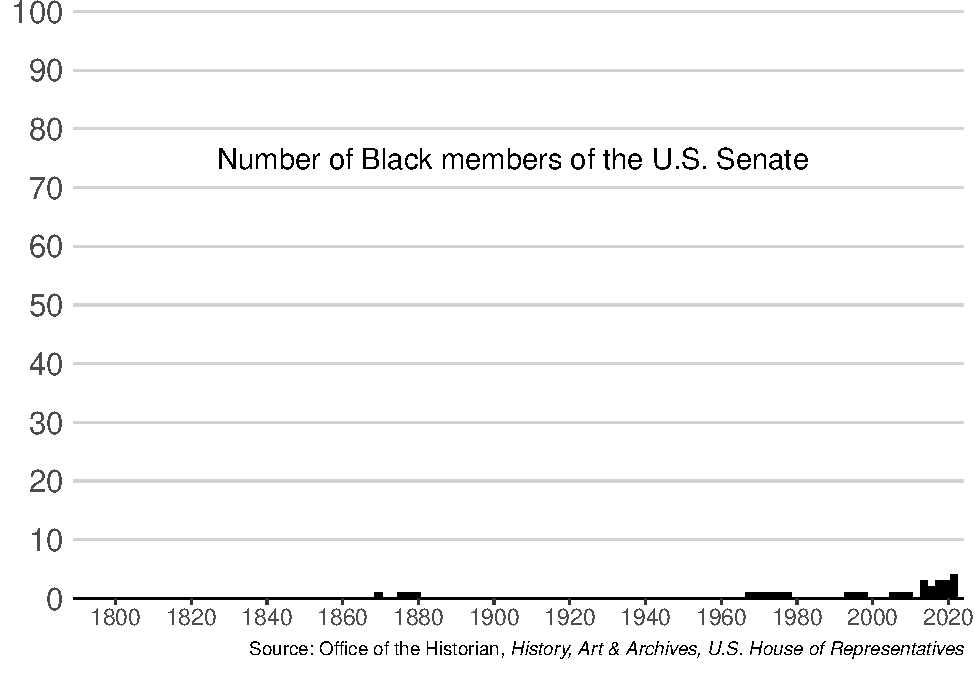
\includegraphics[width=250px]{position_magnitude_files/figure-latex/senators-chart-1} \caption{In this chart, the y-axis limit is the largest possible value, rather than the largest observed value, so plotted values appear to have particularly small magnitudes.}\label{fig:senators-chart}
\end{figure}

\hypertarget{effects-of-axis-limits-on-extraction-of-values}{%
\subsection{Effects of Axis Limits on Extraction of Values}\label{effects-of-axis-limits-on-extraction-of-values}}

The above research consistently demonstrates that the magnitude of \emph{the
difference between values} is interpreted differently depending on the
appearance of the data points when plotted. The present investigation is
concerned with how interpretations of the magnitude of \emph{the values
themselves} are affected by their visual properties. From a cognitive
processing perspective, vertical position is a strong indicator of
magnitude. For example, children appear to intuitively understand the
relationship between height and value \citep{gattis_structure_2002}. Both the
physical world, and language (e.g., spatial metaphors), provide
countless examples where `higher' is associated with `more', and `lower'
with `less', and this principle has been adopted as a convention in data
visualization \citep{tversky_cognitive_1997}.

Research on data visualizations has identified cases where the
relationship between magnitude and vertical position can influence
interpretation. For example, inversions of this mapping in charts can
lead to misinterpretations \citep{okan_when_2012, pandey_how_2015, woodin_conceptual_2022}. Furthermore, when a company's financial
performance was displayed entirely in the bottom fifth of a line chart,
the company was perceived as less successful than when no blank space
appeared above the maximum value \citep{taylor_misleading_1986}.
\citet{sandman_high_1994} investigated assessments of magnitude in risk
ladders, where greater risks are presented at physically higher
positions on a vertical scale. Participants rated the threat of asbestos
exposure higher when it was plotted at a higher position.~

The above findings can be regarded as preliminary evidence that changing
axis limits may affect appraisals of data points' magnitudes. However,
the evidence is not substantial. \citet{taylor_misleading_1986} did not
disclose how judgments were elicited, or provide details of their sample
size. \citet{sandman_high_1994} only explored responses to one specific risk
(asbestos), and each participant only took part in a single trial. In
addition, the `threat' was a composite of several separate ratings,
preventing diagnosis of whether manipulations affected interpretations
of the plotted information in particular, or just related concepts.
Further, both studies introduced a confounding variable by adjusting the
difference between the minimum and maximum y-axis values across
conditions. To understand how different displays of the same values
elicit different inferences about magnitude, and to provide
recommendations for best practice, stronger evidence is required, as is
investigation into the cognitive mechanisms involved in generating these
inferences.~

\hypertarget{the-present-experiments}{%
\subsection{The Present Experiments}\label{the-present-experiments}}

In a set of three experiments employing a large number of observations,
we investigate how employing different axis limits affects
interpretations of the magnitude of plotted values. This manipulation
changes the context surrounding data points, and their physical
positions, but crucially the numerical values themselves remain the
same.

All data visualizations used in the present set of experiments displayed
the chance of negative events occurring. This provides participants with
a purpose in the experiments; evaluating information in such risk
scenarios is a more meaningful task than assessing, in an abstract
manner, how `large' a value is. Furthermore, charts are frequently used
for the communication of such risks, and manipulating aspects of a chart
can change interpretations of the risks displayed
\citep{elting_influence_1999, feldman-stewart_perception_2000, keller_effect_2009, okan_probability_2020, zikmund-fisher_whats_2005}.

Risk events are composed of two core components: 1) chance of occurrence
and 2) outcome magnitude (severity). Individuals' assessments of chance
and severity are not necessarily independent. An event is perceived as
more likely when it is described as having more severe consequences
\citep{harris_estimating_2009, harris_communicating_2011}. In a similar
manner, an event is associated with more substantial consequences when
it is described as more likely \citep{kupor_probable_2020}. One account
suggests that perceptions of probability and outcome magnitude are
related because they are both assumed to reflect the potency of the
event's cause (probability-outcome correspondence principle; \citep{keren_probabilityoutcome_2001}. According to this account,
probabilities can occasionally provide meaningful indications of outcome
magnitude (e.g., rainfall), but it is inappropriate to apply this
perspective to all situations (e.g., volcanic eruptions). Therefore,
even though charts in the present set of experiments only display the
chance of events occurring, assessments of the severity of events'
consequences may also differ between conditions. Collecting separate
judgments of chance and severity of consequences for each scenario
provides a clearer picture of how the manipulation affects distinct
aspects of participants' representations of risk. Use of Likert scales
(with discrete options) rather than visual analogue scales (with
continuous options; \citep{sung_visual_2018}) prevents participants from
simply mapping probability percentages directly onto a linear scale. We
also administered a subjective graph literacy measure, to determine
the degree to which our manipulation(s) affect interpretations after
accounting for differences in graph literacy. Previous
research has shown that responses to visualizations which violate
graphical conventions by using atypical scales suggest individuals with
lower graph literacy are more likely to draw on data
points' physical positions when making inferences about their magnitudes
\citep{okan_how_2016, okan_when_2012}.

\hypertarget{open-research-statement}{%
\subsubsection{Open Research Statement}\label{open-research-statement}}

All experiments in this paper were pre-registered (\url{https://osf.io/qn46s/}). There are no diversions from pre-registered experimental designs, exclusion criteria
or sample size. However, the reported analyses differ in some respects
from the pre-registered protocol. For full transparency, we outline
these diversions here.

Consistent with our pre-registration, when building models for our main
analyses, we sought the most complex random effects structures that
would successfully converge. These model structures were identified by
the \emph{buildmer} package in R \citep{voeten_buildmer_2022}, which subsequently removed terms which did
not contribute substantially to explaining variance in ratings. This
means that the final model used in analysis was not always the most
complex converging model.

In pre-registrations for Experiment 2 and Experiment 3, we proposed
testing for an interaction between our manipulation(s) and graph
literacy. However, this was motivated by a concern about whether
accounting for graph literacy could explain the presence or absence of
effects of our manipulation(s). Therefore, we substitute these planned
analyses with a more appropriate approach, treating graph literacy as a
co-variate only (no interaction). This matches the pre-registered
analysis from Experiment 1, providing consistency across the three
experiments. Due to this revision, pre-registered hypotheses about graph
literacy are not discussed.

\hypertarget{experiment-1}{%
\section{Experiment 1}\label{experiment-1}}

\hypertarget{introduction}{%
\subsection{Introduction}\label{introduction}}

Our initial experiment investigated whether changing axis limits affects
interpretation of data points' magnitudes. For the different versions of
each chart, we presented the same data points at different vertical
positions by altering both the upper and lower y-axis limits.

We predicted that ratings of data points'
magnitudes (chance of occurrence) and/or ratings of the severity of
consequences would be greater when data points were presented at higher
physical positions, compared to when the same data points were presented
at lower positions.

\hypertarget{methods}{%
\subsection{Methods}\label{methods}}

\hypertarget{materials}{%
\subsubsection{Materials}\label{materials}}

Text and an accompanying chart were presented in each trial. Two
sentences outlined a scenario involving a risk, and explained what the
chart depicted. For example:

\begin{quote}
\emph{You are going on a camping trip next week. The graph below shows the
chance of heavy rainfall for three randomly selected days next week.}
\end{quote}

The accompanying dot plot displayed the chance (as a percentage) of a
negative outcome occurring, for three options associated with the
scenario (Figure \ref{fig:example-charts}). The label `Chance' was used
instead of `Probability' to avoid confusion with the standard 0-1 scale
for probabilities, and to reflect casual usage.

\begin{figure}
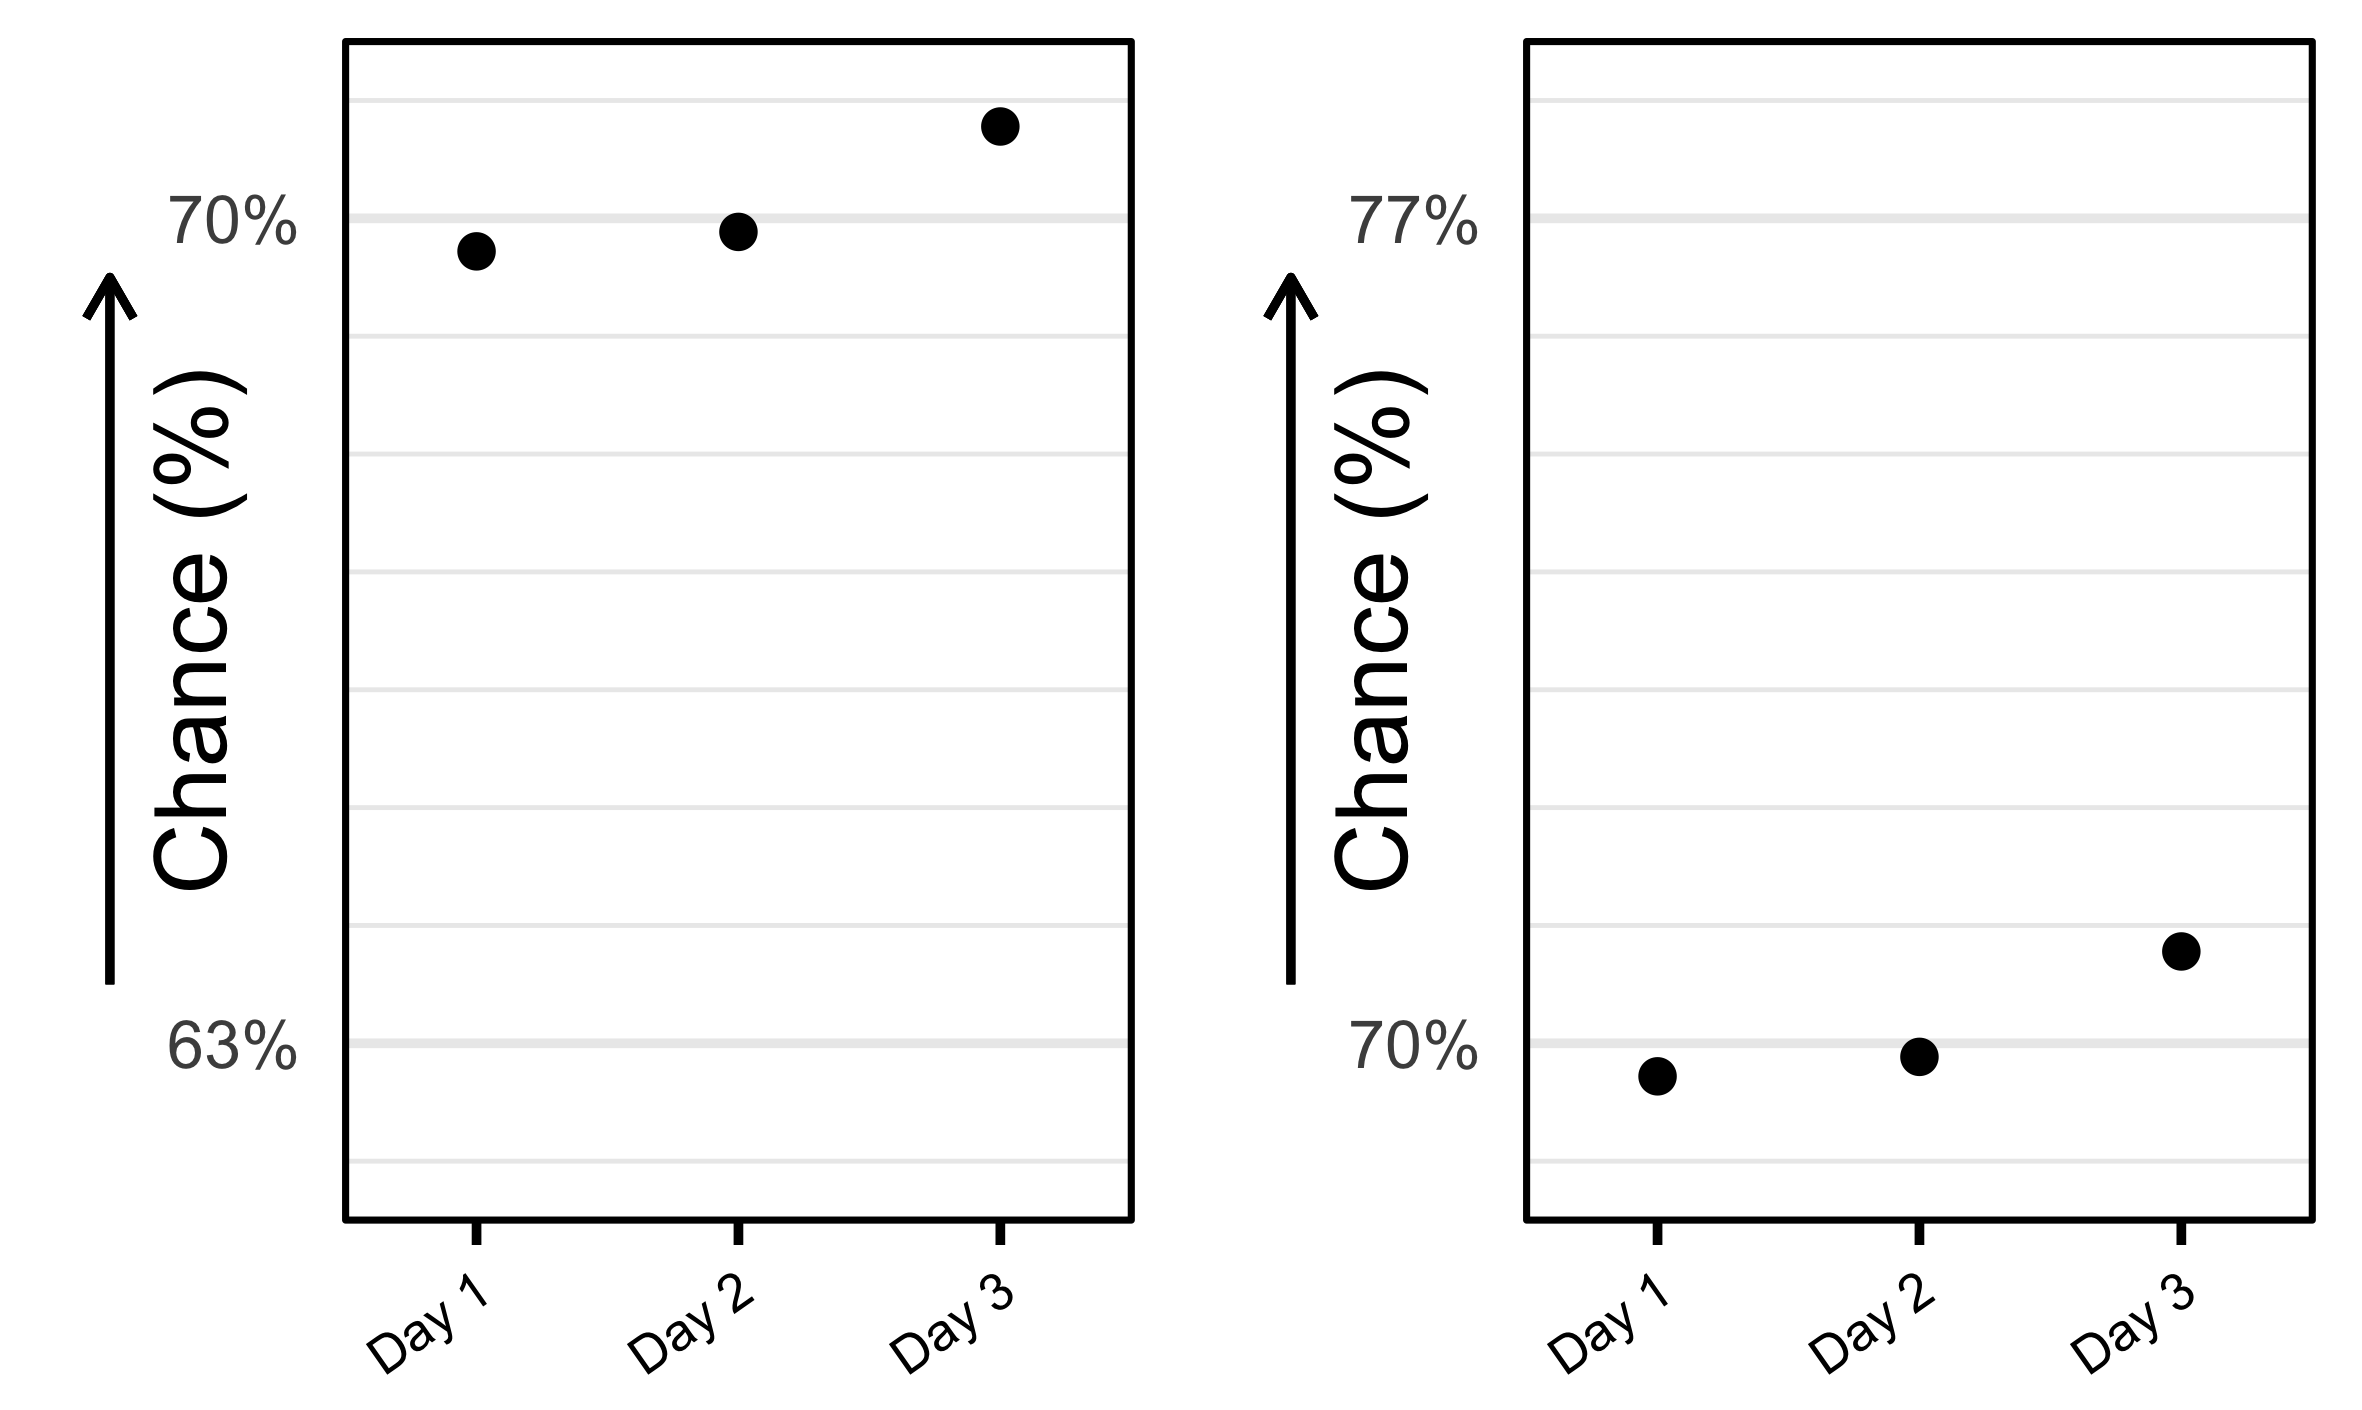
\includegraphics[width=250px]{position_magnitude_files/figure-latex/example-charts-1} \caption{Example Charts. The 'high physical position' condition (left) presents data points near the top of the chart; the 'low physical position' condition (right) presents the same data points near the bottom of the chart.}\label{fig:example-charts}
\end{figure}

In experimental trials (n = 40), all three data points were either
plotted in the top third of the chart (high physical position: Figure
\ref{fig:example-charts}, left) or in the bottom third of the chart
(low physical position: Figure \ref{fig:example-charts}, right). The
plotted dataset differed for each distinct scenario, but was identical
for the two charts associated with a given scenario. In filler trials (n
= 15) and attention check trials (n = 5), data points were plotted in
the middle third of the chart.

The y-axis range in each chart was 10 percentage points. Horizontal
gridlines appeared at one-unit increments. In all trials, the gridline
1.5 percentage points above the bottom of the chart was labelled with a
numerical value, as was the gridline 1.5 percentage points below the top
of the chart.

\hypertarget{procedure}{%
\subsubsection{Procedure}\label{procedure}}

The experiment was programmed in PsychoPy (version 2021.1.4; \citep{peirce_psychopy2_2019}) and hosted on
pavlovia.org. Participants were instructed to complete the experiment on
a desktop computer or laptop, not a tablet or mobile phone. After
providing informed consent, participants submitted their age and gender,
and completed a five-item subjective graph literacy scale
\citep{garcia-retamero_measuring_2016}. They were reminded that the
experiment involved information about risks, and could cause distress,
so were entitled to withdraw from the experiment at any time. Following
this, instructions explained that their task involved assessing the
chance and severity of negative outcomes in various scenarios involving
risks. The instructions noted that some scenarios might appear similar
to other scenarios. Participants were asked to complete the task as
quickly and accurately as possible. Two practice trials were presented
before the experiment proper began.

Two responses were required for each trial: a rating of the chance of
the negative event occurring; and a rating of the severity of the
consequences if that negative event occurred. Above these Likert scales,
a short phrase indicated that the questions should be answered in
response to the plotted data (e.g., \emph{``If you camp on one of these
days\ldots{}''}).

Each Likert scale had two anchors at its extremes, but all other points
were unlabeled. The leftmost option in the `chance' Likert scale was
\emph{`Very unlikely'}, and the rightmost option \emph{`Very likely'}. The
leftmost option in the `severity' Likert scale was \emph{`Very mild'} and the
rightmost option \emph{`Very severe'}. Likert scales appeared on the same
screen as the text and chart (Figure \ref{fig:example-trial}).
Participants were permitted to change their responses as many times as
they wished before proceeding to the next trial, but could not return to
previous trials.

\begin{figure}
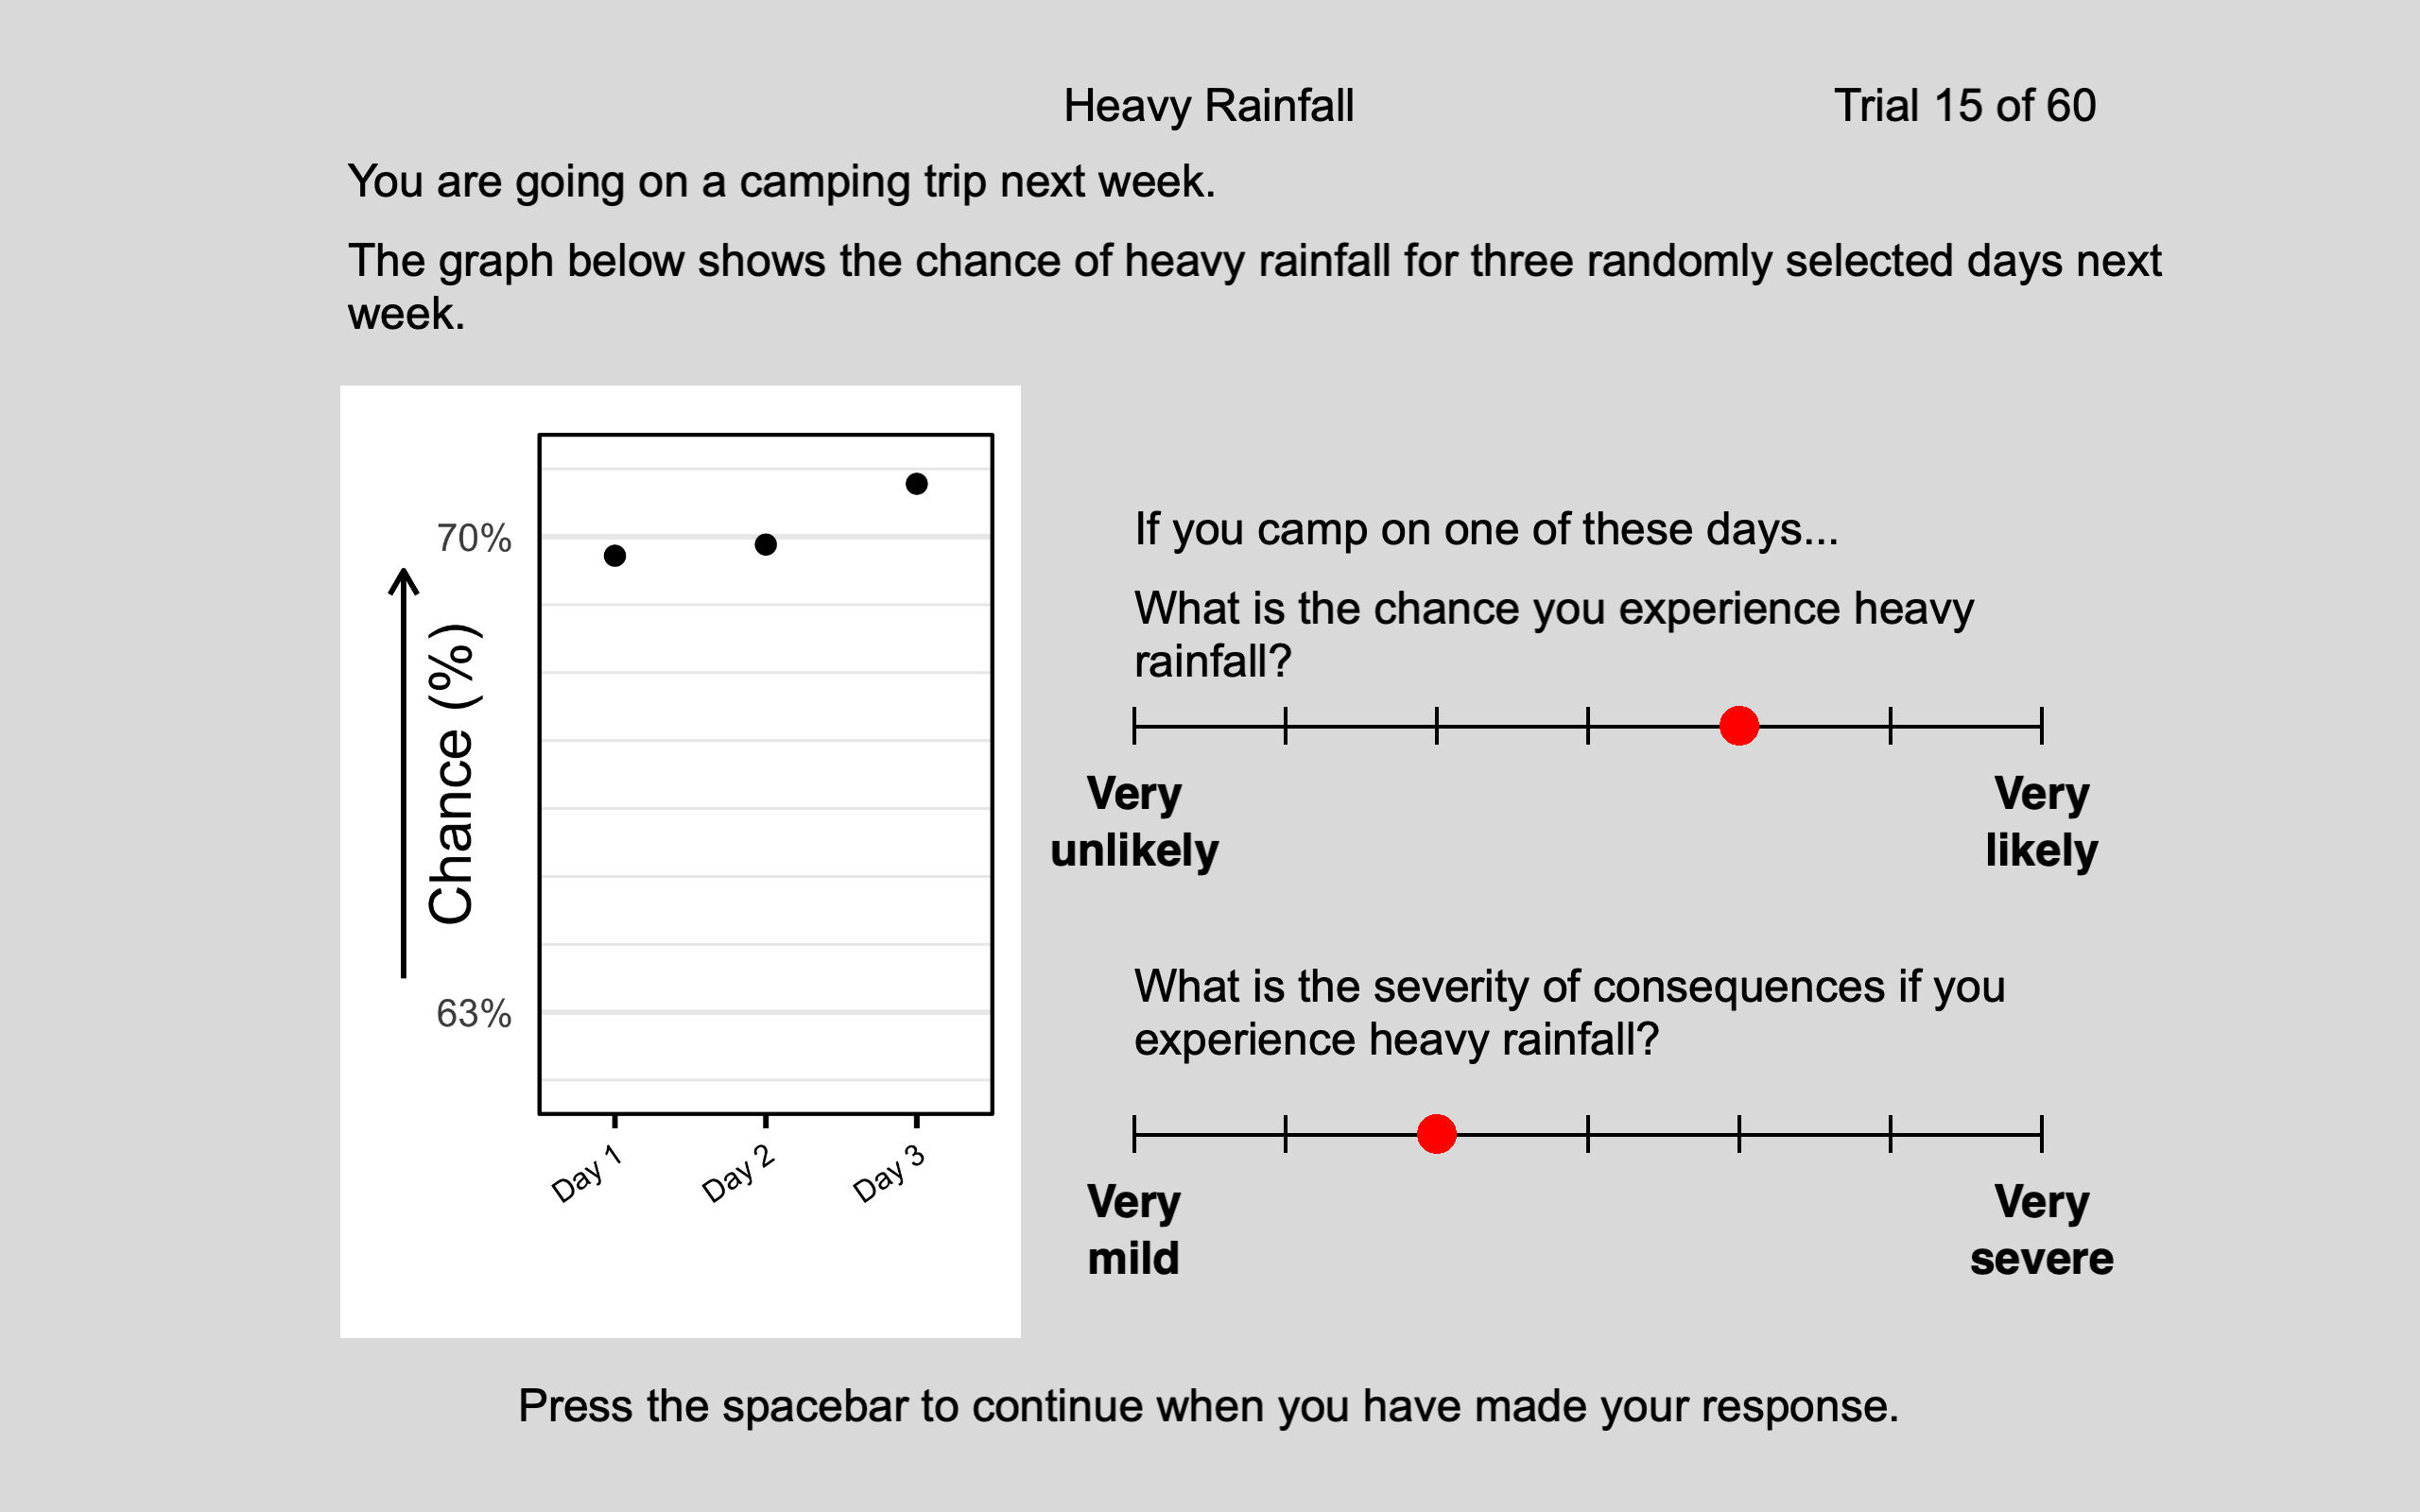
\includegraphics[width=250px]{images/example_trial} \caption{Example Trial. Participants rated the chance and severity of negative outcomes in each trial.}\label{fig:example-trial}
\end{figure}

Attention check trials (n = 5) followed the same layout, with text, a
chart, and Likert scales, but the task differed. Participants were
instructed not to attend to the chart, and instead to provide specified
responses on the Likert scales. For example:

\begin{quote}
\emph{You are expected to stay on task throughout this experiment. For this
trial, ignore the graph below. Respond `Very unlikely' on the top
scale, and `Very mild' on the bottom scale.}
\end{quote}

For attention check trials, the questions above the Likert scales were
\emph{``What is the chance response specified above?''} and \emph{``What is the
severity response specified above?''}.

Before exiting the experiment, participants were informed that all data
presented was fictional and were offered guidance in case of any
distress.

\hypertarget{design}{%
\subsubsection{Design}\label{design}}

We employed a repeated-measures, within-participants design. In
experimental trials, participants encountered each scenario twice: once
with data presented at a high physical position and once with data
presented at a low physical position. In each trial, participants rated
the chance of a negative event occurring, and the severity of its
consequences, on seven-point Likert scales.

Materials were divided into two lists to minimize the likelihood of
different versions of the same scenario appearing in close succession.
In one list, half of the experimental scenarios were accompanied by
charts displaying data at high physical positions, and half were
accompanied by charts displaying data at low physical positions. The
other list contained the alternate versions of each of the experimental
scenarios. Fillers and attention check questions were split between the
two lists, and did not appear more than once. The order of the two lists
was counterbalanced across participants, and within each list, scenarios
were presented in a random order.

\hypertarget{participants}{%
\subsubsection{Participants}\label{participants}}

The experiment was advertised on Prolific.co, a platform for recruiting
participants for online studies. A viral social media post on 24th July
2021 endorsing the website attracted many new users from a narrow
demographic, skewing studies' participant distributions
\citep{charalambides_we_2021}, however, data for this experiment were
collected prior to this. Normal or corrected-to-normal vision and
English fluency were required for participation.

Data were returned by 160 participants. Per pre-registered exclusion
criteria, 10 participants' submissions were rejected because they
answered more than two of 10 attention check questions incorrectly. This
left a total of 150 participants whose submissions were used for
analysis (52.00\% male, 45.33\%
female, 2.67\% non-binary). Mean age was
31.49 (\emph{SD} = 12.47)\footnote{Age data was unavailable for one participant, but was available
  for all other participants in the dataset.}. The mean
graph literacy score was 21.28 (\emph{SD} =
4.58), out of a maximum of 30. Participants
whose submissions were approved were paid £3.55, and average completion
time was 25 minutes \footnote{Timing data was unavailable for two participants, but was
  available for all other participants in the dataset.}. Ethical
approval was granted by The University of Manchester's Division of
Neuroscience \& Experimental Psychology Ethics Committee (Ref.
2021-11115-18258).

\hypertarget{analysis}{%
\subsection{Analysis}\label{analysis}}

Analyses were conducted using R (version 4.1.2, \citep{r_core_team_r_2021}). Raw
data and analysis scripts are available at
\url{https://github.com/duncanbradley/position_magnitude}.

Likert scales only express granularity at the level of ordinal data.
They record whether one rating is higher or lower than than another, but
do not record the magnitude of this difference. Therefore, Likert scales
do not capture values from latent distributions (mental representation)
in a linear manner. On a Likert scale, the distance between one pair of
points and another pair may appear equal, but may represent very
different distances on the latent distribution. Therefore, it is
inappropriate to analyse Likert scale data with metric models, such as
linear regression \citep{liddell_analyzing_2018}. Throughout this paper, we
construct cumulative link mixed-effects models, using the \emph{ordinal}
package (version 2019.12-10, \citep{christensen_ordinalregression_2019}) to analyse Likert scale
ratings.

Selection of random effects structures for models was automated using
the \emph{buildmer} package (version 2.3, \citep{voeten_buildmer_2022}). The maximal random
effects structure included random intercepts for participants and
scenarios, plus corresponding slopes for fixed effects terms
\citep{barr_random_2013}. From this formula, \emph{buildmer} initially identified
the most complex model which could successfully converge, prioritizing
the terms which explained the most variance in the data, then eliminated
terms which did not provide significant contributions (assessed using
likelihood ratio tests).

\begin{figure}
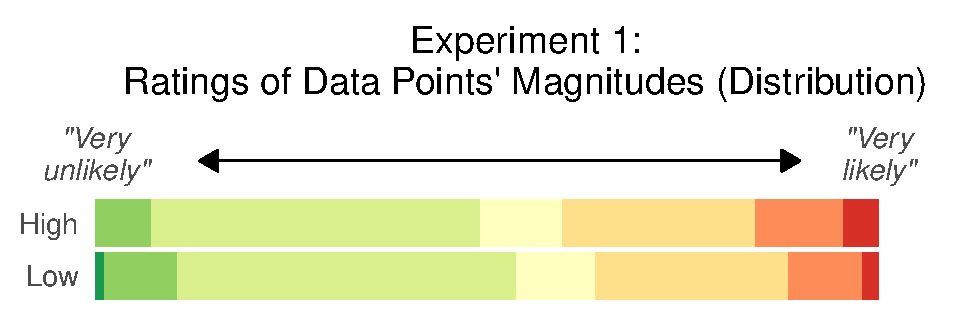
\includegraphics[width=250px]{position_magnitude_files/figure-latex/r1-c-plot-1} \caption{Participants rated the chance of each negative event occurring on a 7-point Likert scale. The distribution of ratings, ranging from "Very unlikely" (far left, dark green) to "Very likely" (far right, red), is shown separately for charts where values were presented at a high physical position (top) and a low physical position (bottom). Note that data points at high physical positions elicited a larger proportion of ratings on the right-hand side (which represents greater magnitudes), compared to data points at low physical positions, which elicited a larger proportion of ratings on the left-hand side (representing smaller magnitudes).}\label{fig:r1-c-plot}
\end{figure}

Figure \ref{fig:r1-c-plot} plots the distribution of participants'
ratings of data points' magnitudes, for data points presented at high
and low physical positions. A likelihood ratio test reveals that a model
including physical position as a fixed effect explains significantly
more variability in ratings than a model which does not include physical
position as a fixed effect (\(\chi^2\)(1) =
74.21, p \textless{} .001). Data
points' magnitudes were rated as greater when those data points were
presented at high physical positions, compared to when the same data
points were presented at low physical positions (z =
8.57, p
\textless{} .001). This model employed random
intercepts for each scenario and each participant. Estimated marginal
means, calculated using the \emph{emmeans} package (version 1.7.0, \citep{lenth_emmeans_2021} for these ratings are plotted in Figure \citet{ref}(fig:r1-c-emm-plot).

For ratings of the severity of consequences, a likelihood ratio test
reveals that a model including physical position as a fixed effect
explains significantly more variability in ratings than a model which
does not include condition as a fixed effect:
(\(\chi^2\)(1) = 6.16, p
= .013). The severity of consequences was
rated as greater when data points representing the chance of an event
occurring were presented at high physical positions, compared to when
the same data points were presented at low physical positions (z =
2.50, p
= .012). This model employed random
intercepts for each scenario, plus random intercepts and slopes for each
participant. The slopes modeled, for each participant, the average
difference between responses to data presented at different positions
(henceforth referred to as `by-position slopes').

We also generate two additional models, to test whether or not the above
results could be explained by differences in graph literacy. These
models were identical to the above models except for the inclusion of
participants' graph literacy scores as an additional fixed effect.
Adjusting for participants' graph literacy scores did not eliminate the
effects of data points' positions on ratings of the magnitude of data
points themselves (z = 8.57, p
\textless{} .001) or severity of
consequences (z = 2.51, p
= .012).

The above analysis employs models with \emph{flexible} thresholds. This
allows for variable distances between decision thresholds in the models
(points on the latent distribution dividing responses between two
categories). Comparison with models that specify \emph{equidistant}
thresholds reveals that models with flexible thresholds are superior,
for ratings of the magnitude of data points themselves
(\(\chi^2\)(4) = 609.44, p
\textless{} .001) and ratings of the severity of
consequences (\(\chi^2\)(4) =
142.84, p \textless{} .001.
flexible). This suggests participants treated
intervals between response categories as irregular, and validates the
use of flexible thresholds in model construction.

\begin{figure}
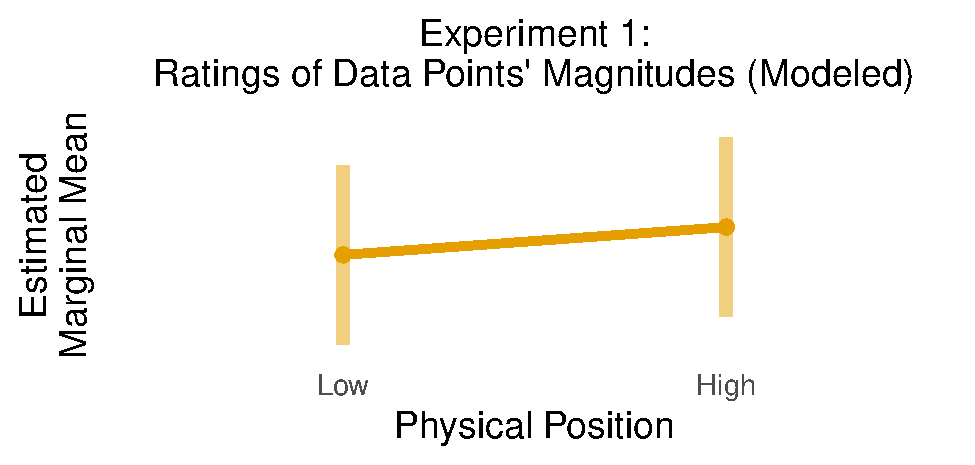
\includegraphics[width=250px]{position_magnitude_files/figure-latex/r1-c-emm-plot-1} \caption{Estimated marginal means for ratings of data points' magnitudes (generated by the cumulative-link mixed model). Magnitudes were rated as greater when data points were presented at high physical positions. Translucent bars show 95\% confidence intervals.}\label{fig:r1-c-emm-plot}
\end{figure}

\hypertarget{discussion}{%
\subsection{Discussion}\label{discussion}}

Participants rated the magnitudes of data points as greater when those
data points were presented near the top of the chart, compared to when
the same data points were presented near the bottom.

Higher bars and ascending lines typically represent higher numbers and
ascending trends, so within a single chart, inferring that values
presented higher up are greater than those lower down will often be
correct in normal usage. This experiment, however, establishes that
inferences about the magnitude of \emph{the same value} can change depending
on its position. Modeling differences in participants' graph literacy
did not remove the influence of our experimental manipulation on
interpretations.

Ratings of both the chance of an event occurring, and the severity of
consequences, were affected by the manipulation of axis limits and data
points' positions, even though the charts only displayed data on the
former. This accords with previous reports of an interplay between
properties of presented information and impressions of related but
distinct concepts, in particular the finding that higher prior
probabilities were associated with impressions of greater event
magnitudes \citep{kupor_probable_2020}. However, it is unclear whether the
effects of different axis ranges on interpretations of magnitude are
driven by an association between a data point's \emph{absolute} position and
its magnitude, or an association between its \emph{relative} position and its
magnitude. If absolute position influences interpretations, mentally
representing the magnitude of a data point may simply involve
associating data points at higher positions with higher values (and
lower positions with lower values). In contrast, if relative position
influences interpretations, mentally representing the magnitude of a
data point would involve a comparison with plausible alternative values,
which are not plotted, but implied through use of blank space. This
important distinction is explored in Experiment 2.

\hypertarget{experiment-2}{%
\section{Experiment 2}\label{experiment-2}}

\hypertarget{introduction-1}{%
\subsection{Introduction}\label{introduction-1}}

Experiment 1 (E1) found that participants associated data points with
greater magnitudes when those data points were positioned near the \emph{top}
of a chart and substantial blank space appeared \emph{below} them, compared
to when the same data points were positioned near the \emph{bottom} of a
chart, with substantial blank space \emph{above}.

One possible explanation for this finding is that participants made
simple associations between absolute position and magnitude, equating
physically higher data points with larger magnitudes and physically
lower data points with smaller magnitudes. This relates to
well-established conceptual metaphors for magnitude, where greater
vertical positions denote greater magnitudes \citep{tversky_cognitive_1997}.

An alternative explanation is that participants used blank space as a
reference point when assessing the magnitude of plotted values. For
example, when viewing substantial blank space above plotted data points,
participants may have recognized the potential for values larger than
those observed, consequently associating plotted data points with
smaller magnitudes.

E1 does not provide a means of differentiating these competing
explanations. Drawing inferences from data points' absolute positions
would orient magnitude judgments in the same direction as drawing
inferences from their positions relative to blank space. A high
magnitude is implied by a data point's high physical position \emph{and} the
presence of substantial blank space below. Therefore, an additional
experiment is required in order to distinguish between the two competing
explanations.~

Inverting a vertical axis changes the relationship between physical
position and numerical value: increasingly \emph{lower} positions represent
increasingly \emph{higher} numerical values. This means data points presented
near the \emph{bottom} of a chart, with substantial blank space above, are
numerically \emph{larger} than the plausible values represented by this blank
space. This is illustrated in Figure \ref{fig:r2-rationale-plot}.
Therefore, inferences invoking blank space would generate the opposite
impressions to inferences invoking data points' physical positions only.

In E2, we manipulate data points' physical positions by changing axis
limits (as in E1), but \emph{also} manipulate axis orientation, by employing
conventional and inverted axes (in a 2 x 2 design). If interpretations
of magnitude differ according to whether data points are smaller or
larger than other plausible values implied by the chart (regardless of
physical position), this will demonstrate that interpretations are
driven by positions relative to blank space, rather by absolute
position.

\begin{figure}
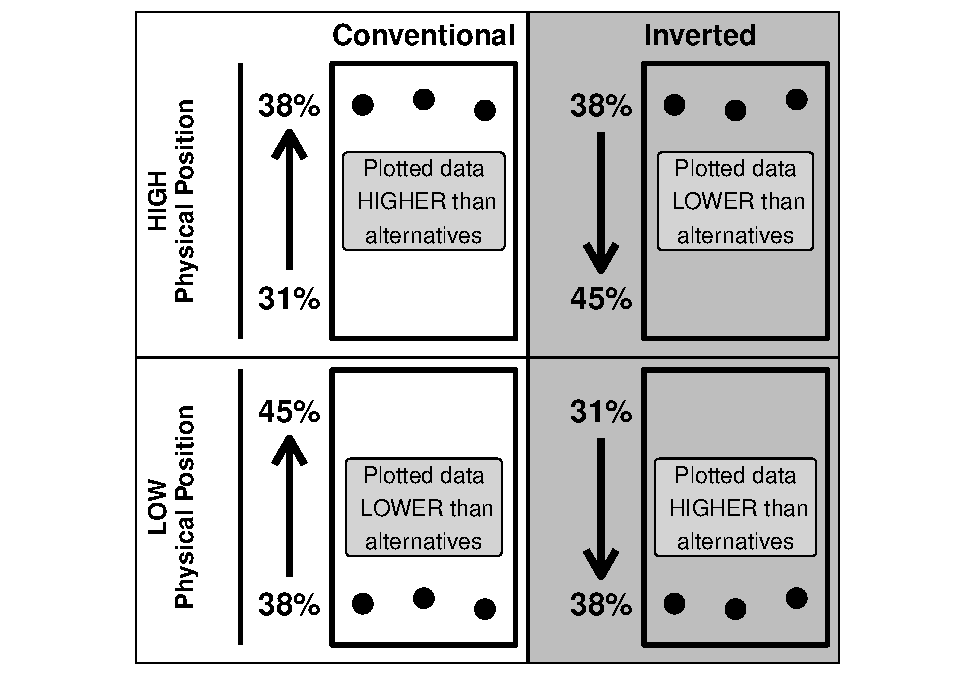
\includegraphics[width=250px]{position_magnitude_files/figure-latex/r2-rationale-plot-1} \caption{Rationale for Experiment 2: Distinguishing the Roles of Absolute and Relative Position. 
 In charts with conventional axis orientations (left column), there is congruity between data points’ absolute positions and their relative positions in the chart. 
 In charts with inverted axis orientations (right column), there is incongruity between data points’ absolute positions and their relative positions in the chart. 
 For example, at high absolute positions in conventional charts (top left), data points are relatively higher than implied alternatives. But at the same absolute positions, in inverted charts, the same values are relatively lower than alternatives (top right).}\label{fig:r2-rationale-plot}
\end{figure}

Previous research suggests that charts with inverted axes can be prone
to misinterpretation when viewers are not informed about the inversion
(\citet{pandey_how_2015}; \citet{woodin_conceptual_2022}). In E2, we provide explicit
instruction to ensure participants are aware that inverted charts are
presented.

For charts with conventional axis orientations,
we predicted in our pre-registration that results from E1 would be replicated. That is, data
points presented at higher physical positions would be associated with
greater magnitude ratings, compared to data points presented at lower
physical positions. For charts with inverted axis orientations, we
outlined what different patterns of magnitude ratings would signal about
the mechanism used to interpret magnitude. Specifically, use of absolute
position would be indicated by greater magnitude ratings for data points
at \emph{higher} physical positions (and therefore no difference compared to
conventional charts). Alternatively, use of position relative to blank
space would be indicated by greater magnitude ratings for data points at
\emph{lower} physical positions (and therefore the opposite pattern compared
to conventional charts).

\hypertarget{method}{%
\subsection{Method}\label{method}}

\hypertarget{materials-1}{%
\subsubsection{Materials}\label{materials-1}}

For this experiment, we used a Latin-squared design where participants
only viewed one chart per scenario. In response to this, we increased
the number of scenarios. This provided some compensation for the reduced
experimental power caused by a reduction the number of observations per
participant (as well as a reduction in participant numbers).

Two scenarios which were fillers in E1 were used as experimental
scenarios\footnote{For one of these scenarios, the mean of the plotted data was also
  modified.} and three additional scenarios were created. One filler
scenario was removed due to a concern about its quality (it concerned
the risk to others as well as the risk to oneself). This gave a total of
24 experimental scenarios, 12 filler scenarios, and 5 attention check
questions (41 trials in total).

\hypertarget{procedure-1}{%
\subsubsection{Procedure}\label{procedure-1}}

The experiment was programmed in PsychoPy (version 2021.2.3 \citet{peirce_psychopy2_2019}). Participants specified the highest level of education they had received,
in addition to answering demographic questions on age and gender. An
additional slide in the instructions explained how to identify and
interpret the different axis orientations, and encouraged participants
to pay attention to this:

\begin{quote}
\emph{You should pay attention to the direction of the arrow on the
`Chance' axis. If the arrow points upwards, the numbers in the graph
get bigger as the axis goes up. Alternatively, if the arrow points
downwards, the numbers get bigger as the axis goes down.}
\end{quote}

Otherwise, the procedure was identical to E1.

\hypertarget{design-1}{%
\subsubsection{Design}\label{design-1}}

We employed a Latin-squared, within-participants design. Participants
encountered each individual scenario only once, but were exposed to all
combinations of position and axis orientation throughout the experiment.

\hypertarget{participants-1}{%
\subsubsection{Participants}\label{participants-1}}

The experiment was not advertised on Prolific.co to those who had
participated in E1, or those who signed-up to Prolific.co after 24th
July 2021 (due to the shift in participant demographics). Normal or
corrected-to-normal vision and English fluency were required for
participation.

Data were returned by 129 participants. Per pre-registered exclusion
criteria, five participants' submissions were rejected because they
answered more than two of 10 attention check questions incorrectly.
Submissions from four other participants were excluded from the final
dataset for the following reasons: maximum completion time (67 minutes)
was exceeded (two participants); the submission constituted second
attempt following a saving error on first attempt (one participant);
data were collected prior to pre-registration (one participant). This
left a total of 120 participants whose submissions were used in the
analysis (49.17\% male, 50.83\%
female). Mean age was 29.32 (\emph{SD} =
10.45). 100\% had
completed at least secondary education. The mean graph literacy score
was 21.73 (\emph{SD} =
4.70). Participants whose submissions were
approved were paid £2.37, and average completion time was
21 minutes. Ethical approval was
granted by The University of Manchester's Division of Neuroscience \&
Experimental Psychology Ethics Committee (Ref. 2021-11115-20464).

\hypertarget{analysis-1}{%
\subsection{Analysis}\label{analysis-1}}

\begin{figure}
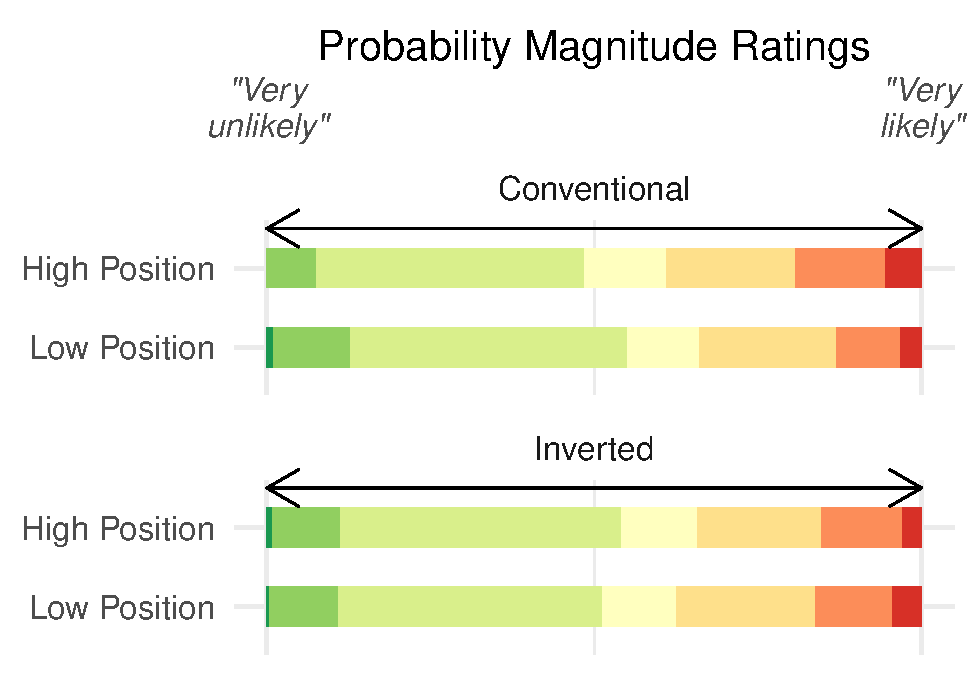
\includegraphics[width=250px]{position_magnitude_files/figure-latex/r2-c-plot-1} \caption{Participants rated the chance of each negative event occurring on a 7-point Likert scale. The distribution of ratings, ranging from "Very unlikely" (far left, dark green) to "Very likely" (far right, red) is shown separately for each combination of the levels of each condition (axis orientation: conventional, inverted; data points' physical position: high, low). Note that the pattern of responses to data presented at different positions in the Conventional Axis condition appears to be the opposite to the pattern for Inverted Axis condition. When charts used conventional axes, greater magnitude ratings were more common for data presented at high physical positions, whereas when charts used inverted axes, greater magnitude ratings were more common for data presented at low physical positions.}\label{fig:r2-c-plot}
\end{figure}

Figure \ref{fig:r2-c-plot} plots the distribution of participants'
ratings of data points' magnitudes, for data points presented at high
and low physical positions, in charts with conventional axis
orientations and inverted axis orientations. A likelihood ratio test
reveals that a model including the interaction between physical position
and axis orientation as a fixed effect explains significantly more
variability in ratings than a model without this interaction as a fixed
effect (\(\chi^2\)(1) = 8.22, p
= .004). There was a significant
interaction between physical position and y-axis orientation (z =
2.91, p
= .004). This
interaction is plotted in Figure \ref{fig:r2-int-plot}. This model
employed random intercepts and by-position slopes for each scenario.
Random intercepts were included for each participant, as well as slopes
capturing differences in participants' responses to data presented at
different positions, different orientations, and the interaction between
these.

Pairwise comparisons (with Sidak adjustment) reveal that the effect of
position in charts with conventional y-axis orientations (E1) was
replicated (z = 3.56, p
= .001). Data points'
magnitudes were rated as greater when they were presented at high
physical positions, compared to when they were presented at low physical
positions. There was no significant difference between magnitude ratings
for data points plotted at different positions when inverted axes were
used (z = -1.39, p
= .512). Therefore, we
observe a different pattern of results when an inverted axis is used,
compared to when a conventional axis is used. This suggests that
differences in ratings for data points at different positions in
physical space are not due to simple associations between vertical
position and magnitude. The interaction remained when controlling for
graph literacy: z = 2.91, p
= .004, and when controlling for
list number: z = 2.92, p
= .004.

For ratings of the severity of consequences, a likelihood ratio test
reveals that a model including the interaction between physical position
and axis orientation as a fixed effect explains significantly more
variability in ratings than a model without this interaction as a fixed
effect (\(\chi^2\)(1) = 5.13, p
= .024).There was a significant
interaction between physical position and y-axis orientation (z =
2.28, p
= .022). This
model employed random intercepts for each scenario. Random intercepts
were included for each participant, as well as slopes capturing
differences in participants' responses to data presented at different
positions, different orientations, and the interaction between these.
Despite the interaction, the main effect in severity ratings from E1,
different responses to data points at different positions in
conventional charts, was not replicated
(1.53, p
= .414). There was also
no evidence of different responses to data points at different positions
in inverted charts (-1.54, p
= .412). This
interaction appears to be driven by a weak and likely spurious
difference between ratings for data points at high physical positions in
inverted and conventional charts (-2.52,
p = .047). The
interaction remained when controlling for graph literacy: z =
2.29, p
= .022, and when controlling for
list number: z = 2.28, p
= .023.

Models employing flexible decision thresholds (as above) were superior
to models employing equidistant thresholds, for ratings of the magnitude
of data points themselves (\(\chi^2\)(4) =
346.93, p \textless{} .001), and
ratings of the severity of consequences:
(\(\chi^2\)(4) = 74.10, p
\textless{} .001).

\begin{figure}
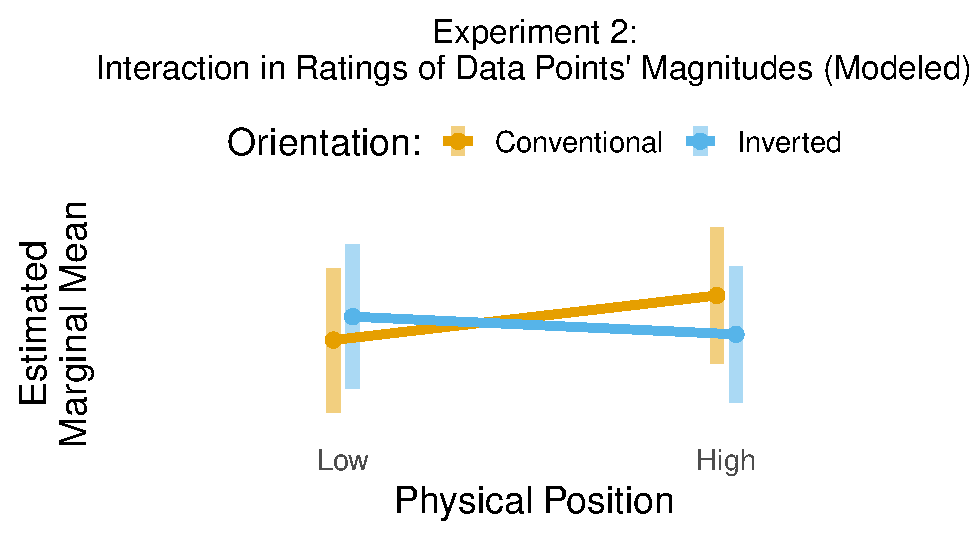
\includegraphics[width=250px]{position_magnitude_files/figure-latex/r2-int-plot-1} \caption{Estimated marginal means for ratings of data points' magnitudes (generated by the cumulative-link mixed model). The slope for conventional charts differs from the slope of inverted charts. Thus, the effect of position on interpretation of data points' magnitudes differs according to axis orientation. Translucent bars show 95\% confidence intervals.}\label{fig:r2-int-plot}
\end{figure}

\hypertarget{discussion-1}{%
\subsection{Discussion}\label{discussion-1}}

In E1, when using conventional charts only, we found that displaying
data within different axis limits affected magnitude judgments. However,
it was unclear whether judgments were based on data points' absolute
positions, or their positions relative to blank space, because both
would generate similar interpretations. Therefore, in E2, for half of
trials, we reversed the mapping of values in physical space, so these
two features would imply different magnitudes for a given value.

In E2, we replicated the primary finding from E1. In charts with
conventional axis orientations, the same data points elicited different
chance judgments when presented at different positions. These
differences were consistent with magnitudes implied by data points'
absolute positions and their positions relative to blank space. However,
in charts with inverted axis orientations, the same pattern was not
observed. Therefore, we can conclude that interpretations of magnitude
are affected by a chart's physical arrangement of values. The pattern of
differences in magnitude judgments for data points presented at distinct
physical positions depends on how axes are oriented.

Figure \ref{fig:r2-int-plot} suggests that the pattern of results for
inverted charts is the reverse of the pattern for conventional charts.
However, our analysis indicates that the same data points did not elicit
significantly different magnitude judgments when presented at different
positions in \emph{inverted} charts. Therefore, we cannot conclude from this
analysis that magnitude judgments are driven solely by data points'
positions relative to blank space. The lack of significant difference is
likely due to a lack of experimental power. An additional experiment is
required to confirm whether there is a genuine difference.

\hypertarget{experiment-3}{%
\section{Experiment 3}\label{experiment-3}}

\hypertarget{introduction-2}{%
\subsection{Introduction}\label{introduction-2}}

The interaction in E2 revealed that the influence of position on
magnitude judgments depends on how different numerical values are
arranged in a chart (axis orientation). The pattern of responses in
inverted charts appeared to be the inverse of the pattern for
conventional charts. This suggests that participants may not have based
inferences about magnitude on data points' absolute positions, but on
their positions relative to blank space. However, the absence of a
significant difference between ratings for data points at different
positions in inverted charts prohibits the conclusion that
interpretations are driven entirely by comparisons with plausible values
implied by blank space.

It is possible that no significant effect was detected due to
insufficient experimental power. Unlike E1, with 150 participants in a
single-factor design, E2 involved 120 participants in a Latin-squared 2
x 2 design. Despite an increase in the number of experimental scenarios
(from 20 to 24), there were still fewer observations for each unique
condition (3000 in E1 vs.~720 in E2).

In E3 we increase the experimental power and focus only on inverted
charts. This will provide a clearer account of how magnitude is
interpreted in inverted charts, furthering understanding of the
mechanism by which axis ranges influence interpretations of magnitude.

We outlined in our pre-registration what
different patterns of magnitude ratings would signal about the
mechanisms used to interpret magnitude. Specifically, use of absolute
position would be indicated by higher magnitude ratings for data points
at \emph{high} physical positions (mirroring the finding for conventional
charts). Alternatively, use of position relative to blank space would be
indicated by higher magnitude ratings for data points at \emph{low} physical
positions (the reverse of the finding for conventional charts).

\hypertarget{method-1}{%
\subsection{Method}\label{method-1}}

\hypertarget{materials-2}{%
\subsubsection{Materials}\label{materials-2}}

Materials were identical to E1, except for the inversion of the y-axis
in all charts, including practice trials. There were 60 trials in total
(40 experimental trials, 15 fillers, 5 attention check questions).

\hypertarget{procedure-2}{%
\subsubsection{Procedure}\label{procedure-2}}

The experiment was programmed in PsychoPy (version 2021.2.3 \citet{peirce_psychopy2_2019}). As in E2, participants were asked to indicate their education level. One
slide in the instructions explained to participants how charts with
inverted axes function: \emph{``In all graphs in this experiment, the arrow on
the `Chance' axis points downwards, meaning the numbers get bigger as
the axis goes down.''}. Otherwise, the procedure was identical to E1.

\hypertarget{design-2}{%
\subsubsection{Design}\label{design-2}}

As in E1, we employed a repeated-measures, within-participants design.
Participants encountered each experimental scenario twice: once with
data presented at a high physical position and once with data presented
at a low physical position.

\hypertarget{participants-2}{%
\subsubsection{Participants}\label{participants-2}}

The experiment was not advertised on Prolific.co to those who had
participated in E1 or E2, or those who signed-up to Prolific.co after
24th July 2021. Normal or corrected-to-normal vision and English fluency
were required for participation.

Data were returned by 161 participants. Per pre-registered exclusion
criteria, 10 participants' submissions were rejected because they
answered more than two of 10 attention check questions incorrectly. One
additional participant was excluded from the final dataset because they
exceeded the maximum completion time (87 minutes). This left a total of
150 participants whose submissions were used for analysis:
(60.00\% male, 40.00\% female).
Mean age was 29.64 (\emph{SD} =
9.56)\footnote{Age data was unavailable for two participants, but was available
  for all other participants in the dataset.}. 100\% had
completed at least secondary education. The mean graph literacy score
was 21.87 (\emph{SD} =
4.28). Participants whose submissions were
approved were paid £3.45, and average completion time was
24 minutes. Ethical approval was
granted by The University of Manchester's Division of Neuroscience \&
Experimental Psychology Ethics Committee (Ref. 2021-11115-20745).

\hypertarget{analysis-2}{%
\subsection{Analysis}\label{analysis-2}}

Figure \ref{fig:r3-c-plot} plots the distribution of participants'
ratings of data points' magnitudes, for data points presented at
different physical positions in inverted charts.

\begin{figure}
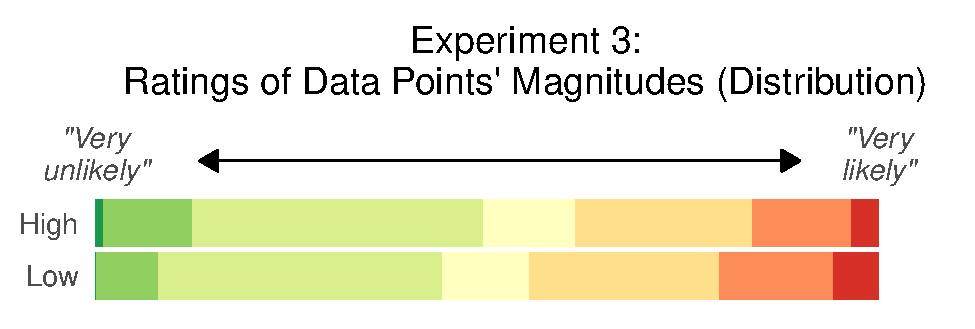
\includegraphics[width=250px]{position_magnitude_files/figure-latex/r3-c-plot-1} \caption{Participants rated the chance of each negative event occurring on a 7-point Likert scale. The distribution of ratings, ranging from "Very unlikely" (far left, dark green) to "Very likely" (far right, red), is shown separately for charts where values were presented at a high physical position (top) and a low physical position (bottom). Note that data points at high physical positions elicited a larger proportion of ratings on the left-hand side (which represents smaller magnitudes), compared to data points at low physical positions, which elicited a larger proportion of ratings on the right-hand side (representing greater magnitudes).}\label{fig:r3-c-plot}
\end{figure}

A likelihood ratio test
reveals that a model including physical position as a fixed effect
explains significantly more variability in ratings of data points' magnitudes than a model which
does not include physical position as a fixed effect
(\(\chi^2\)(1) = 46.45, p
\textless{} .001). Data points' magnitudes were
rated as greater when those data points were presented at low physical
positions, compared to when the same data points were presented at high
physical positions (z = 6.80, p
\textless{} .001). This model employed random intercepts for each
scenario. This effect remained when adjusting for participants' graph
literacy scores (z = 6.83, p
\textless{} .001). Estimated marginal means
for these ratings are plotted in Figure \ref{fig:r3-c-emm-plot}.

For ratings of the severity of consequences, a likelihood ratio test
reveals that a model including physical position as a fixed effect did
not explain significantly more variability in ratings than a model
without this fixed effect (\(\chi^2\)(1) =
3.40, p = .065). This
model employed random intercepts for each scenario, plus random
intercepts and by-position slopes for each participant. This finding
remained when adjusting for participants' graph literacy scores (z =
1.85, p
= .064).

Models employing flexible decision thresholds (as above) were superior
to models employing equidistant thresholds, for ratings of the magnitude
of data points themselves (\(\chi^2\)(4) =
752.74), and ratings of the severity of consequences
(\(\chi^2\) (4) = 177.78, p
\textless{} .001).

\begin{figure}
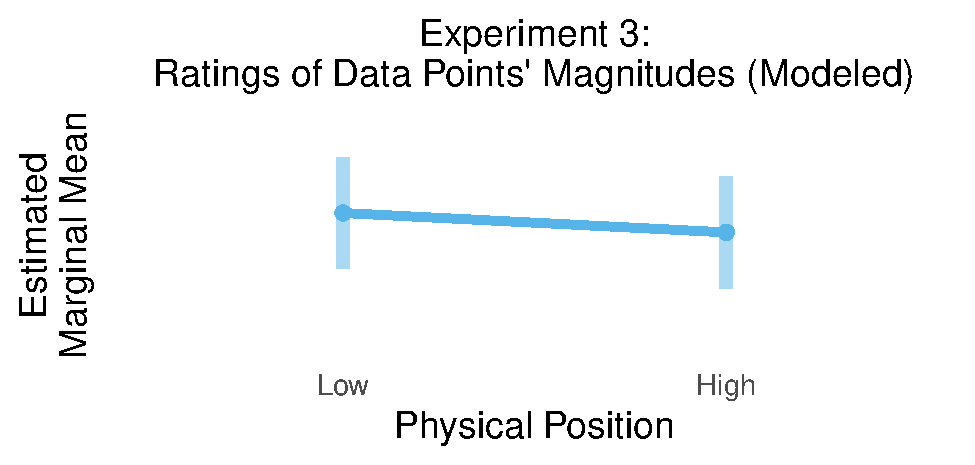
\includegraphics[width=250px]{position_magnitude_files/figure-latex/r3-c-emm-plot-1} \caption{Estimated marginal means for ratings of data points' magnitudes (generated by the cumulative-link mixed model). Magnitudes were rated as greater when data points in inverted charts were presented at low physical positions. Translucent bars show 95\% confidence intervals.}\label{fig:r3-c-emm-plot}
\end{figure}

\hypertarget{discussion-2}{%
\subsection{Discussion}\label{discussion-2}}

When viewing charts with inverted axes, participants judged data points'
magnitudes according to whether accompanying blank space implied the
existence of higher or lower plausible values. Participants ignored
conventional associations between position and magnitude to interpret
magnitude in the context of the chart.

In the previous experiment (E2), we did not observe a significant
difference between magnitude ratings for data points at different
positions in inverted charts, although the pattern was consistent with
the use of blank space in the interpretation of the plotted data.
However, E3, with increased experimental power, demonstrates that such a
difference is statistically significant.

E2 involved switching between conventional and inverted charts, whereas
E3 presented inverted charts in isolation. However, the differences in
estimated marginal means for inverted charts, which represent the
differences in ratings of data points' magnitudes when presented at
different positions, are almost identical for these two experiments (E2:
0.34; E3:
0.33). This suggests inverted charts
were not treated differently in the different experiments. Therefore,
the presence or absence of switching should not prohibit the use of E3's
data in explaining E2's interaction.

In light of this, we can interpret the results of E2 more easily. The
same data points, presented at the same positions in a chart, convey
different magnitudes depending on how they compare to plausible values
implied by blank space. Viewers do not draw upon simple associations
between vertical position and magnitude, but recognize the context in
which values are plotted.

\hypertarget{general-discussion}{%
\section{General Discussion}\label{general-discussion}}

Over three experiments, we demonstrate how judgments of data points'
magnitudes are influenced by the presence of blank space in a chart.
Regardless of their physical positions, data points were associated with
greater magnitudes when they were numerically greater than the plausible
values represented by blank space. This was observed for charts with
both conventional and inverted axes. This highlights viewers'
sensitivity to context in the interpretation of information in data
visualizations, suggesting designers should consider this aspect when
creating charts.

When comparing data points within a single chart, it is appropriate to
infer that data points which appear at different positions between two
axis limits have distinct magnitudes. The results we report indicate
that magnitude judgments can vary when \emph{the same value} appears at
different positions between two axis limits. Interpretation of an
absolute value is biased by its relative position.~

The impact of surrounding information on assessments of data is an
example of a framing effect. We illustrate that this effect occurs in
the absence of contrasting data points: the presence of blank space is
sufficient for implying the relative status of plotted data.

The present data complement findings from prior research on y-axis
truncation, which has found that the choice of axis limits can impact
interpretation of data. The results we report reinforce the notion that
the amount of blank space surrounding plotted values influences viewers'
impressions of those values. While previous investigations have shown
that y-axis limits affect \emph{comparisons} of plotted values
\citep{correll_truncating_2020, witt_graph_2019, yang_truncating_2021}, the
present findings show that they also affect \emph{magnitude judgments}.

A previous study addressing a similar question also concluded that a
data point's location within a range of values affects interpretation of
its magnitude \citep{sandman_high_1994}. The present set of experiments
builds upon this research by identifying the mechanism behind this
effect and removing the confound of variable axes ranges. It also
extends the finding beyond a single scenario to a wider range of
situations, and separately analyses specific judgments, rather than
using a combined measure, to verify that different presentations affect
judgments of the specific variable plotted in a chart.

This set of experiments was not concerned with endorsing or opposing
inverted charts; the sole function of these charts was in distinguishing
competing explanations. However, when explicit instruction was provided,
our data provide evidence of comprehension, contrary to the typical
finding of misinterpretation resulting from associating higher positions
with higher values \citep{woodin_conceptual_2022, pandey_how_2015}.

Visualization rhetoric involves presenting numerical information in a
way that provokes a particular interpretation
\citep{hullman_visualization_2011}. The manipulation of visualization
components examined in the present set of experiments is related to two
rhetorical strategies: \emph{axis thresholding} and \emph{contrast.} The former is
an instance of `information access' rhetoric, and involves setting an
axis range that provides an incomplete picture of the data. The latter
is an instance of `mapping' rhetoric, and employs visual properties to
promote comparisons.

We did not find consistent evidence that assessments of the severity of
consequences are affected by the positioning of values representing the
chance of events occurring. Prior research has found that probability
estimates change as a function of outcome magnitude
\citep{harris_communicating_2011, harris_estimating_2009} and that outcome
magnitude estimates change as a function of event probability
\citep{kupor_probable_2020}. However, whereas prior research focused on the
potency of an event, we asked participants to evaluate another feature:
the severity of its consequences. How affected parties are impacted by
an event is one step removed from a core component of risk, outcome
magnitude. In addition, unlike prior work which substantially
manipulated underlying scenarios, our more subtle manipulation retained
the same probability values, changing only the surrounding context. The
effect of relative position on interpretation of chance data does not
consistently extend to judgments about the severity of consequences.

Adjusting for data visualization literacy did not remove the influence
of axis range on interpretations. \citet{yang_truncating_2021} also observed
that data visualization literacy could not sufficiently explain variance
in the degree of bias caused by y-axis truncation. This measure captures
comprehension of the conventions of data visualization, indicating
receipt of elementary instruction \citep{okan_how_2016}. Therefore, it is
perhaps better suited to measuring ability to decipher more complicated
designs, but is not well-placed to predict susceptibility to differences
in presentation format \citep{yang_truncating_2021}.

\hypertarget{implications-for-visualization-design}{%
\subsection{Implications for Visualization Design}\label{implications-for-visualization-design}}

This finding highlights an opportunity for data visualization designers
to creatively construct axes for dramatic effect. Introducing blank
space when setting axis limits allows designers to persuasively convey
large or small magnitudes. However, even those avoiding creative use of
blank space should be sensitive to our finding that axis ranges are
likely to be considered representative of relevant values for assessing
the magnitude of plotted data. Designers should consider what is \emph{not}
plotted and reflect on the impression(s) of magnitude resulting from
their choice of axis limits. To avoid misleading displays, axes should
present appropriate values. Like \citet{correll_truncating_2020}, we
acknowledge that there is no objectively correct method for achieving
this. Ultimately, the designer decides what context is appropriate,
based on the chart's purpose and content. This may involve taking into
account historical data, comparable scenarios, established baselines,
current objectives, \emph{etc.}. Our findings are also relevant for assessing
the quality of data visualizations; one should consider whether a chart
appropriately portrays magnitude, in addition to standard
considerations.

Setting an axis range that extends far beyond the range of the plotted
data impacts discrimination ability \citep{witt_graph_2019}, and may distract
attention from meaningful variance within the data. Witt recommends
setting an axis range to 1.5-2 times the plotted data's standard
deviation. This guidance is broadly consistent with our suggestions in
its recommendation that axis limits should take into account relevant
values to provide context. The present experiment has demonstrated that
magnitude is communicated by the relative position of data points within
the space of all plausible values.

When following Witt's \citep{witt_graph_2019} suggestions, data points'
positions are determined solely by the size of the numerical difference
between two conditions. A large difference between conditions would
result in data points being located near the two extremes of the chart,
which may capture genuine small and large magnitudes. At other times,
applying Witt's guidance will create an inaccurate impression of
individual magnitudes. For example, with a small difference between
conditions, no data points will be displayed near the extremes, even
though they may be genuinely large or small when considered within a
larger context. This occurs because Witt's guidance was created for the
sole purpose of managing bias and sensitivity when comparing two
conditions (in fields with standardized effect sizes). Accordingly,
setting axes which provide context for \emph{individual} magnitudes, is not
considered pertinent. Again, designers must consider their dataset and
the message they intend to relate in order to reach a trade-off between
suitable communication of variability and individual magnitudes. A
possible compromise may involve displaying values against blank space to
convey magnitude in context, and also in a focused display to facilitate
comparisons between values. This resembles an approach for communicating
differences discussed by \citet{correll_truncating_2020}, and reported to
benefit users by \citet{ritchie_lie_2019}. Its suitability for conveying
magnitude should be investigated in future work.

\hypertarget{limitations}{%
\subsection{Limitations}\label{limitations}}

To avoid likelihood of misinterpretation, participants were given
instructions on how to read inverted charts. This may have suppressed a
spontaneous interpretation of magnitude, based on physical position, in
favor of a learned interpretation. Our investigation therefore only
explains how viewers interpret magnitude when they know how to interpret
a given chart.

In addition to associations between vertical position and magnitude,
vertical position is also a common conceptual metaphor for emotional
valence. Lower physical positions are typically associated with negative
valence and higher physical positions with positive valence.
\citet{woodin_conceptual_2022} found that comprehension is facilitated when the
physical arrangement of data is consistent with the conceptual metaphor
for valence, but that associations between vertical position and
numerical magnitude affect interpretations more strongly. In the present
set of experiments, charts displayed negative outcomes, so data were
aligned with the conceptual metaphor for valence in inverted charts, and
misaligned in conventional charts. Participants evidently did not use
valence metaphors to interpret values in conventional charts; this would
have produced the opposite pattern of results to those observed. The
simplest explanation for our results is that participants relied on
relative position when interpreting both conventional and inverted
charts, rather than sometimes generating inferences based on a
conceptual metaphor for valence.

In analyses employing graph literacy as a co-variate, graph literacy
scores were calculated as the average of five Likert scale responses.
This means that responses to graph literacy questions were modeled as
continuous data, whereas Likert scale ratings from experimental trials
were modeled as ordinal data. This approach was used by the scale's
developers \citep{garcia-retamero_measuring_2016}, but is not the most
appropriate method \citep{liddell_analyzing_2018}.

\hypertarget{conclusion}{%
\subsection{Conclusion}\label{conclusion}}

The position of data points in a chart affects interpretation of how big
or small their values are. We demonstrate that this relationship between
physical position and inferences about magnitude critically depends on
whether accompanying blank space represents higher or lower alternatives
to the plotted data. Viewers take into account the context in which data
appears, even when comparison values are not explicitly displayed. Axis
limits and blank space warrant consideration from data visualization
designers.

\hypertarget{acknowledgments}{%
\section*{Acknowledgments}\label{acknowledgments}}
\addcontentsline{toc}{section}{Acknowledgments}

Duncan Bradley was supported by the Economic and Social Research Council
(Grant Number ES/P000665/1). This work was supported in part by a BPS
Cognitive Section Postgraduate Rapid Project Grant. We thank Jen McBride
and Paul Warren for comments on an earlier draft, and Paul Stott for
assistance with manuscript formatting.

\setlength{\bibsep}{0.0pt}

%\bibliographystyle{bib_styles/abbrv}
\bibliographystyle{bib_styles/abbrvnatdoi}
%\bibliographystyle{bib_styles/abbrv-doi}
%\bibliographystyle{bib_styles/abbrv-doi-narrow}
%\bibliographystyle{bib_styles/abbrv-doi-hyperref}
%\bibliographystyle{bib_styles/abbrv-doi-hyperref-narrow}

{\fontsize{8pt}{9.6pt}\selectfont \bibliography{bibliography}}
\end{document}
